 \chapter{Risultati computazionali} \label{chap:risultati}

% **************************** Define Graphics Path **************************
\ifpdf
    \graphicspath{{Chapter7/Figs/Raster/}{Chapter7/Figs/PDF/}{Chapter7/Figs/}}
\else
    \graphicspath{{Chapter7/Figs/Vector/}{Chapter7/Figs/}}
\fi

\section{Costruzione delle istanze di prova}

\section{Risultati}
Abbiamo preso in considerazione due tipologie di istanze, basate sui set di posizioni $P$ e illustrate in \figurename\ \ref{figP}, rappresentanti diversi scenari. \\
La prima tipologia consiste in griglie quadrate o rettangolari complete, ovvero in cui in ogni punto interno è possibile posizionare un drone. La seconda tipologia invece (griglie $btn25$, $btn41$, $btn48$ \cite{degioPal2013}) include posizioni vietate, dette no-flight zones, causate per esempio da ostacoli o divieti di sorvolo. \\
%
\begin{figure}
	\begin{center}
		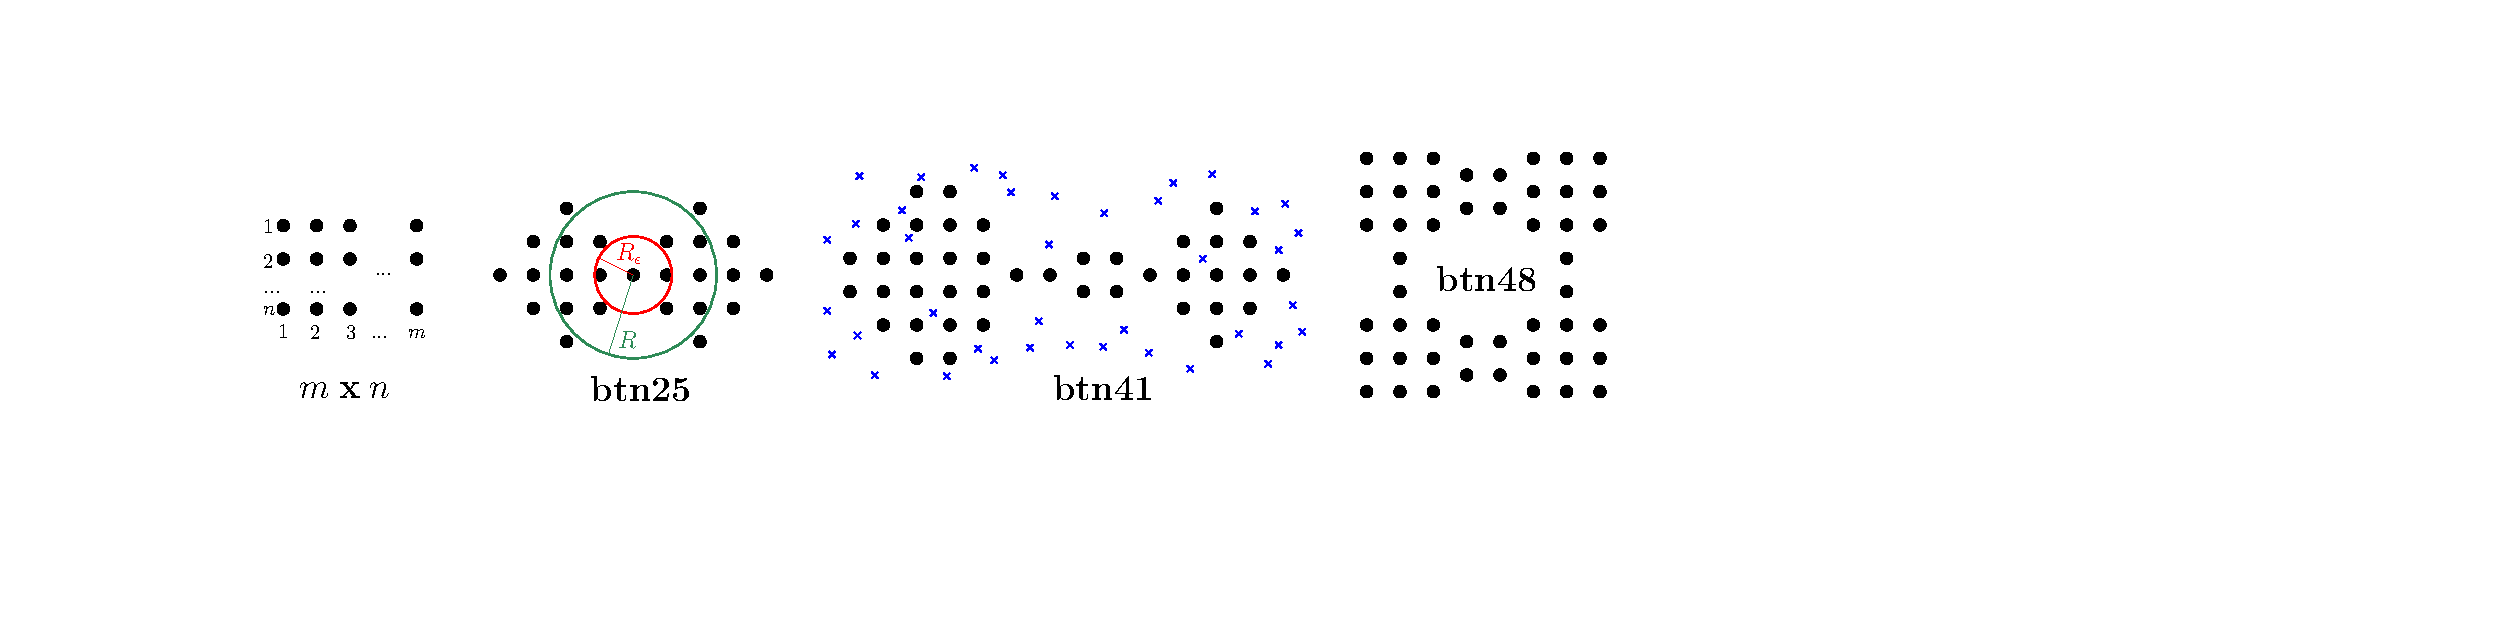
\includegraphics[scale=0.60]{figTopolHorUsersP}
	\end{center}
	\caption{Tipologie di griglie utilizzate.} \label{figP}
\end{figure}
%
Le posizioni degli utenti sono state generate in maniera casuale attorno all'area della griglia, con maggiore probabilità attorno ai bordi (ad esempio, le croci blu in \figurename\ \ref{figP}), assicurandosi che tutti i client si trovassero a distanze minori di $R$ da ciascun punto $i \in P$, per evitare istanze impossibili da risolvere a causa del cattivo posizionamento. \\
Test preliminari per il dimensionamento del dataset hanno dimostrato l'impossibilità di risolvere istanze, con i vincoli temporali e di memoria stabiliti, con più di 30 clients. \\ Per ogni griglia e per ogni numero di utenti nell'insieme $\{10, 20, 30\}$ sono state generate 3 istanze casuali, generando in maniera casuale le posizioni degli utenti e le matrici di traffico. \\ 
Come detto nel \chaptername\ \ref{cap:metodi}, il modello è stato implementato in C++ utilizzando le CPLEX Callable Library (C API), con tempo massimo di esecuzione di 40 minuti, parallelismo deterministico e focus sull'ottimizzazione della memoria.Le istanze sono state risolte su un sistema con 4 processori Intel Xeon E5520 @2.27 GHz e 32 GB di RAM. \\
I risultati ottenuti con questo campione del dataset sono mostrati in \tablename \ref{tabRes}. La prima colonna indica il nome della griglia (o la sua dimensione, in numero di punti potenziali, in formato lunghezza x altezza) e il numero di utenti,la seconda colonna si riferisce all'elaborazione con CPLEX, e le restanti due alle euristiche. La colonna Time indica il tempo medio delle tre istanze, la colonna Best il miglior tempo registrato, la colonna Drones il numero di droni minimo necessario.  \\
Dai risultati possiamo vedere che mentre l'euristica Binary Y perde praticamente sempre contro i risultati CPLEX, l'euristica Set Y presenta performance estremamente migliori nella maggior parte dei casi. \\  

\setlength{\tabcolsep}{3.5 pt}
\renewcommand\arraystretch{1.1}
\begin{table} 
	\scriptsize
	\center
	\begin{tabular}{lc|rrr|rrr|rrr}
		\hline
		\multicolumn{2}{c}{\bf Instance} & \multicolumn{3}{|c}{{\bf Cplex 12.6}} & \multicolumn{3}{|c}{{\bf Binary Y}} & \multicolumn{3}{|c}{{\bf Set Y}}\\
		{\bf $P$} & $|V|$ & Time & Best & Drones & Time & Best & Drones & Time & Best & Drones \\
		\hline
		4x8 & 10 & 0.3 & 0.3 & 5 & 0.7 & 0.4 & 4 & 0.2 & 0.1 & 4 \\
		4x8 & 20 & 5.0 & 4.8 & 7 & 9.5 & 7.1 & 8 & 3.6 & 3.4 & 8 \\
		4x8 & 30 & T.L. & T.L. & 32 & T.L & T.L. & 32 & T.L. & T.L. & 32 \\
		6x6 & 10 & 0.42 & 0.4 & 4 & 0.7 & 0.5 & 4 & 0.3 & 0.2 & 4 \\
		6x6 & 20 & 10.3 & 8.9 & 8 & 19.0 & 18.3 & 9 & 8.3 & 7.2 & 8 \\
		6x6 & 30 & T.L. & T.L. & 36 & T.L. & T.L. & 32 & T.L. & T.L. & 32 \\
		9x9 & 10 & 3.25 & 2.8 & 4 & 3.0 & 2.38 & 10 & 3.2 & 2.6 & 4 \\
		9x9 & 20 & T.L. & T.L. & 81 & T.L. & T.L. & 81 & T.L. & T.L. & 81 \\
		9x9 & 30 & T.L. & T.L. & 81 & T.L. & T.L. & 81 & T.L. & T.L. & 81 \\
		btn25 & 10 & 1.03 & 0.9 & 4 & 1.5 & 0.9 & 4 & 0.45 & 0.4 & 4 \\
		btn25 & 20 & 22.5 & 20.8 & 4 & T.L. & T.L. & 25 & T.L. & T.L. & 25 \\
		btn25 & 30 & T.L. & T.L. & 25 & T.L. & T.L. & 25 & T.L. & T.L. & 25 \\
		btn41 & 10 & 7.2 & 4.2 & 4 & 9.2 & 8.3 & 6 & 5.1 & 3.8 & 6 \\
		btn41 & 20 & T.L. & T.L. & 41 & T.L. & T.L. & 3 & T.L. & T.L. & 41 \\
		btn41 & 30 & T.L. & T.L. & 41 & T.L. & T.L. & 3 & T.L. & T.L. & 41 \\
		btn48 & 10 & 1.42 & 1.2 & 4 & 4.1 & 3.9 & 4 & 1.1 & 1.5 & 4 \\
		btn48 & 20 & 32.5 & 30.4 & 4 & T.L. & T.L. & 48 & T.L. & T.L. & 48 \\
		btn48 & 30 & T.L. & T.L. & 48 & T.L. & T.L. & 48 & T.L. & T.L. & 48 \\
		5x10 & 10 & 0.7 & 0.7 & 4 & 1.2 & 0.5 & 5 & 0.8 & 0.5 & 4 \\
		5x10 & 20 & 22.7 & 18.9 & 4 & T.L. & T.L. & 50 & T.L. & T.L. & 50 \\
		5x10 & 30 & T.L. & T.L. & 50 & T.L. & T.L. & 50 & T.L. & T.L. & 50 \\
		6x15 & 10 & 4.6 & 3.3 & 4 & 6.6 & 4.4 & 6 & 5.6 & 4.7 & 6 \\
		6x15 & 20 & T.L. & T.L. & 4 & T.L. & T.L. & 90 & T.L. & T.L. & 90 \\
		6x15 & 30 & T.L. & T.L. & 90 & T.L. & T.L. & 3 & T.L. & T.L. & 90 \\
		\hline
	\end{tabular}
	\normalsize
	\caption{Risultati sperimentali} 
	\label{tabRes}
\end{table}
%